\section{Klassendiagramme Web}
\subsection{VOTEsso und Configurations}
\begin{figure}[htp]
	\centering
	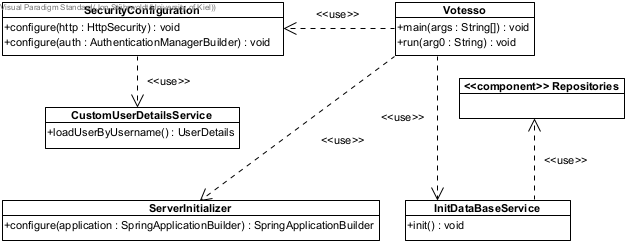
\includegraphics[width=\textwidth]{img/classvotesso.png}	
	\caption{Klassendiagramm - Configurations}
	\label{fig:klassendiagramm-vote}
\end{figure}

\begin{table}[htp]
	\centering
	\begin{tabularx}{\textwidth}{X X}
		\rowcolor[HTML]{C0C0C0} 
		\textbf{Klassenname} & \textbf{Aufgabe} \\
		Votesso & Main-Klasse, über die das Programm gestartet werden kann. \\
		\rowcolor[HTML]{E7E7E7}
		SecurityConfiguration & Verwaltet den Zugriff auf URLs.   \\
		 CustomUserDetailsService &  Kümmert sich um die Autorisierung, beim Login von Administratoren. \\
		 \rowcolor[HTML]{E7E7E7}
		ServerInitializer & Konfiguriert und baut die Anwendung. \\
		InitDataBaseService & Initialisiert alle Repositries mit dem jeweiligen Datenbankinhalt.  \\
	\end{tabularx}
	\caption{Klassenbeschreibung - Web, Configurations}
	\label{table:klassenbeschreibung-web-configurations}
\end{table}


\subsection{Model}
\begin{figure}[H]
	\centering
	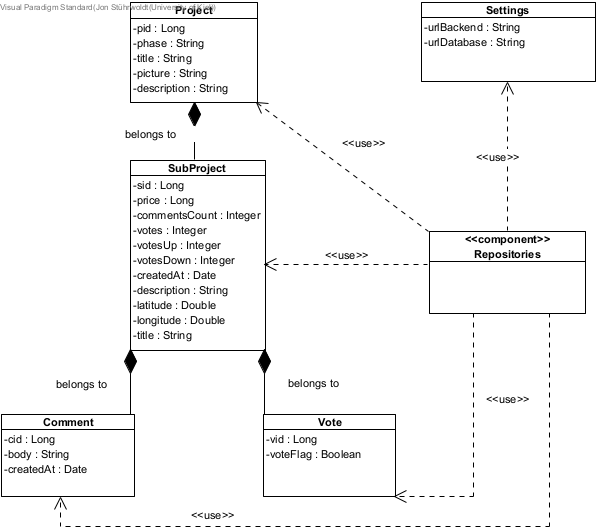
\includegraphics[width=\textwidth]{img/classmodel.png}	
	\caption{Klassendiagramm - Model}
	\label{fig:klassendiagramm-model}
\end{figure}

\begin{table}[H]
	\centering
	\begin{tabularx}{\textwidth}{X X}
		\rowcolor[HTML]{C0C0C0} 
		\textbf{Klassenname} & \textbf{Aufgabe} \\
		Project & Klasse, die den Datentypen Project repräsentiert und alle nötigen Informationen eines (Haupt-)Projekts enthält. Der Aufbau der Klasse dient als Vorlage für die Objekte, die im zugehörigen Repository abgespeichert werden. \\
		\rowcolor[HTML]{E7E7E7} 
		 SubProject &  Klasse, die den Datentypen SubProject repräsentiert und alle nötigen Informationen eines TeilProjekts enthält. Der Aufbau der Klasse dient als Vorlage für die Objekte, die im zugehörigen Repository abgespeichert werden. \\
		Comment & Klasse, die den Datentypen Comment repräsentiert und alle nötigen Informationen eines Kommentars enthält. Der Aufbau der Klasse dient als Vorlage für die Objekte, die im zugehörigen Repository abgespeichert werden. \\
		\rowcolor[HTML]{E7E7E7} 
		Vote & Klasse, die den Datentypen Vote repräsentiert und alle nötigen Informationen einer Abstimmung/Bewertung enthält. Der Aufbau der Klasse dient als Vorlage für die Objekte, die im zugehörigen Repository abgespeichert werden. \\
		Settings & Klasse, die die URLs enthält, welche durch den Administrator konfigurierbar sind. Von dieser Klasse soll später lediglich eine Instanz existieren. Der Aufbau der Klasse dient als Vorlage für das eine Objekt, welches im zugehörigen Repository abgespeichert wird.  \\
	\end{tabularx}
	\caption{Klassenbeschreibung - Web, Model}
	\label{table:klassenbeschreibung-web-model}
\end{table}

\subsection{Repositories}
\begin{figure}[H]
	\centering
	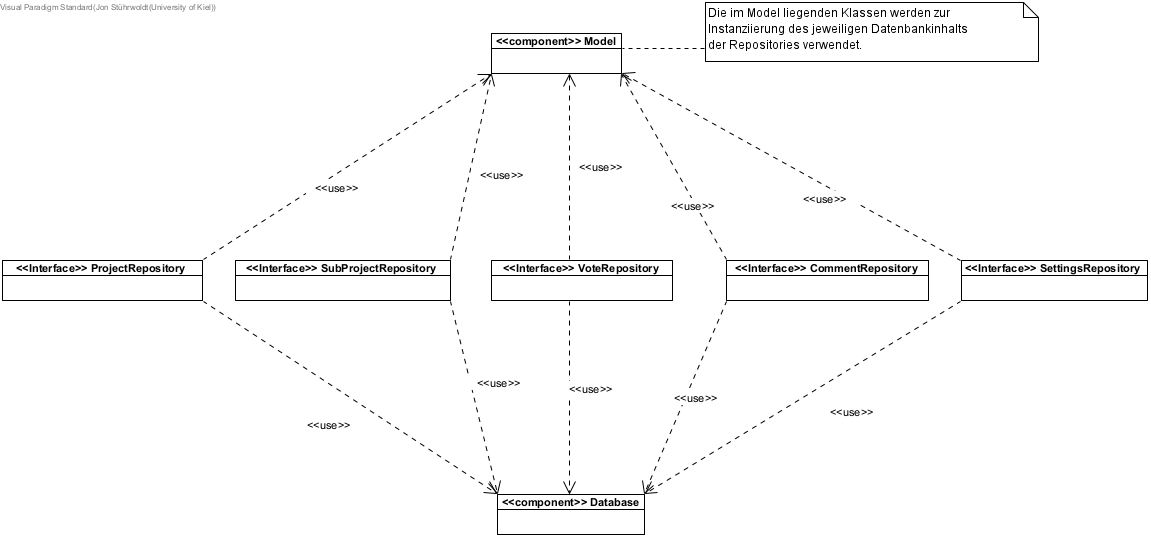
\includegraphics[width=\textwidth]{img/classrepo.png}	
	\caption{Klassendiagramm - Repositories}
	\label{fig:klassendiagramm-repo}
\end{figure}

\begin{table}[H]
	\centering
	\begin{tabularx}{\textwidth}{X X}
		\rowcolor[HTML]{C0C0C0} 
		\textbf{Klassenname} & \textbf{Aufgabe} \\
		ProjectRepository & Interface, welches die Verwaltung von Objekten des Datentyps Project übernimmt. \\
		\rowcolor[HTML]{E7E7E7}
		SubProjectRepository & Interface, welches die Verwaltung von Objekten des Datentyps SubProject übernimmt.  \\
		 VoteRepository &  Interface, welches die Verwaltung von Objekten des Datentyps Vote übernimmt. \\
		 \rowcolor[HTML]{E7E7E7}
		CommentRepository & Interface, welches die Verwaltung von Objekten des Datentyps Comment übernimmt. \\
		SettingsRepository & Interface, welches die Verwaltung der einen Instanz der Klasse Settings übernimmt.  \\
	\end{tabularx}
	\caption{Klassenbeschreibung - Web, Repositories}
	\label{table:klassenbeschreibung-web-repositories}
\end{table}

Die Interfaces werden durch das Spring Boot Framework realisiert.


\subsection{Controller}
\begin{figure}[H]
	\centering
	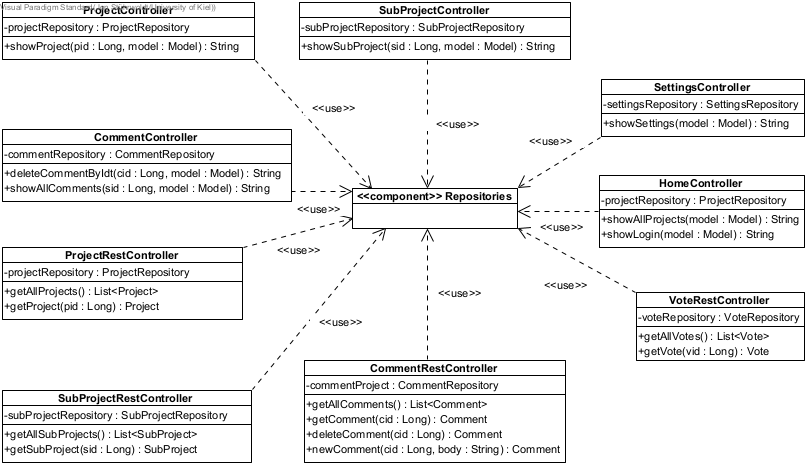
\includegraphics[width=\textwidth]{img/controller.png}	
	\caption{Klassendiagramm - Controller}
	\label{fig:klassendiagramm-cont}
\end{figure}

\begin{table}[H]
	\centering
	\begin{tabularx}{\textwidth}{X X}
		\rowcolor[HTML]{C0C0C0} 
		\textbf{Klassenname} & \textbf{Aufgabe} \\
		HomeController & Klasse, die eine HTML-Seite zurückgibt, die eine Liste aller (Haupt-)Projekte enthält und dem Administrator die Möglichkeit bietet, über einen Button auf die Login-Seite weitergeleitet zu werden. \\
		\rowcolor[HTML]{E7E7E7}
		ProjectController & Klasse, die eine HTML-Seite zurückgibt, welche alle Informationen eines Projektes enthält. Zu diesen Informationen zählt unter anderem eine Liste der zugehörigen Teilprojekte, in der die jeweiligen Seiten der Teilprojekte verinkt sind.  \\
		 SubProjectController &  Klasse, die eine HTML-Seite zurückgibt, die alle Informationen eines Teilprojektes und einen Link zu den Kommentaren dieses Teilprojektes enthält. \\
		 \rowcolor[HTML]{E7E7E7}
		CommentController & Klasse, die eine HTML-Seite zurückgibt, die alle Kommentare eines gegebenen Teilprojektes enthält. Administratoren haben auf dieser Seite außerdem die Möglichkeit Kommentare zu löschen. \\
		SettingsController & Klasse, die eine HTML-Seite zurückgibt, auf welcher Administratoren die System-URLs konfigurieren können.  \\
		\rowcolor[HTML]{E7E7E7}
		ProjectRestController & Klasse, die Methoden für den Austausch von Projekten mit der App über die Rest-API bereitstellt.  \\
		 SubProjectRestController &  Klasse, die Methoden für den Austausch von Teilprojekten mit der App über die Rest-API bereitstellt. \\
		 \rowcolor[HTML]{E7E7E7}
		CommentRestController & Klasse, die Methoden für den Austausch von Kommentaren mit der App über die Rest-API bereitstellt. \\
		VotesRestController & Klasse, die Methoden für den Austausch von Bewertungen/Abstimmungen mit der App über die Rest-API bereitstellt.  \\
	\end{tabularx}
	\caption{Klassenbeschreibung - Web, Controller}
	\label{table:klassenbeschreibung-web-controller}
\end{table}

\section{Klassendiagramm App}

\begin{figure}[H]
	\centering
	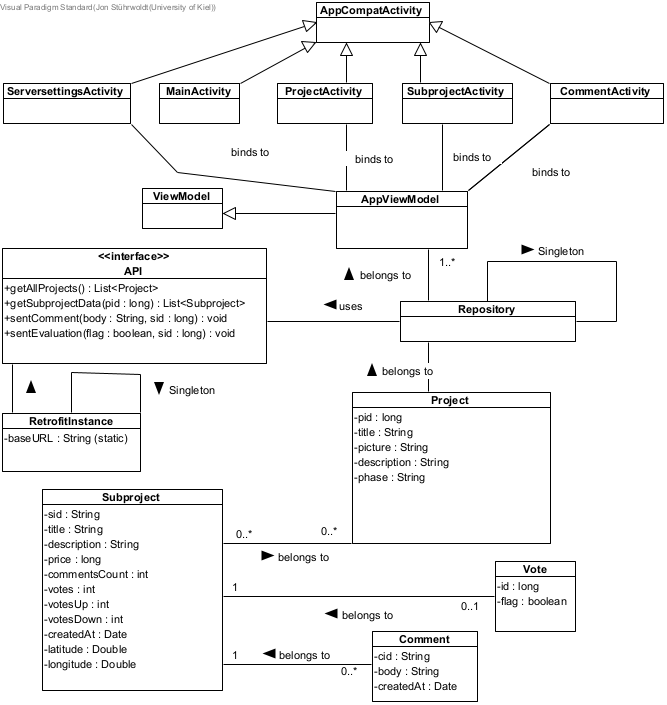
\includegraphics[width=\textwidth]{img/classapp.png}	
	\caption{Klassendiagramm - App}
	\label{fig:klassendiagramm-app}
\end{figure}

\begin{table}[H]
	\centering
	\begin{tabularx}{\textwidth}{X X}
		\rowcolor[HTML]{C0C0C0} 
		\textbf{Klassenname} & \textbf{Aufgabe} \\
		AppCompatActivity &Von Android bereitgestellte Basisklasse für Activities. \\
		\rowcolor[HTML]{E7E7E7}
		MainActivity & Realisiert die Projektübersichtsseite, Startpunkt unserer App. \\
		 Serversettingsactiivity & Realisiert die Server-Einstellungsseite. Hier kann die URL des Backend angepasst werden. \\
		 \rowcolor[HTML]{E7E7E7}
		ProjectActivity & Realisiert die Projektdetailseite und die Auflistung der Teilprojekte. \\
		SubprojectActivity & Realisiert die Teilprojektseite mit einem Kommentareingabebereich.\\
		\rowcolor[HTML]{E7E7E7}
		CommentActivity & Realisiert die Auflistung aller zu dem Teilprojekt geschriebenen Kommentare.  \\
		AppViewModel & Stellt das Bindeglied zwischen View und Model dar.  Verarbeitet die vom Repository erhaltenen Daten und stellt es der View bereit.  \\
		\rowcolor[HTML]{E7E7E7}
		 Viewmodel &  Von Android bereitgestellte Basisklasse für unser AppViewModel. \\
		Repository & Ist für den Datenaustausch zwischen App und Backend zuständig. Die Repository-Klasse tätigt sämtliche API-Calls. \\
		\rowcolor[HTML]{E7E7E7}
		RetrofitInstance & Klasse, um API-Calls mittels http zu realisieren.  \\
		APIService & Benötigtes Interface für Aufrufe an das Backend (nötig für Retrofit).\\
		\rowcolor[HTML]{E7E7E7}
		Project & Klasse für das Projekt.\\
		Subproject & Klasse für das Teilprojekt.\\
		\rowcolor[HTML]{E7E7E7}
		Comment & Klasse für den Kommentar.\\
		Vote & Klasse, die die Evaluierung der Teilprojekte erleichtert.\\
	\end{tabularx}
	\caption{Klassenbeschreibung - App}
	\label{table:klassenbeschreibung-web-controller}
\end{table}